
\title{ConvNet Lab for DD2427}
\author{
        Miquel Marti Rabadan\\921019-1459\\miquelmr@kth.se
}
\date{\today}

\documentclass[12pt]{article}

\usepackage{graphicx,palatino}

\begin{document}
\maketitle

\section{ConvNet building blocks}
\subsection{Convolution}

\begin{figure}[htbp]
 \centering
 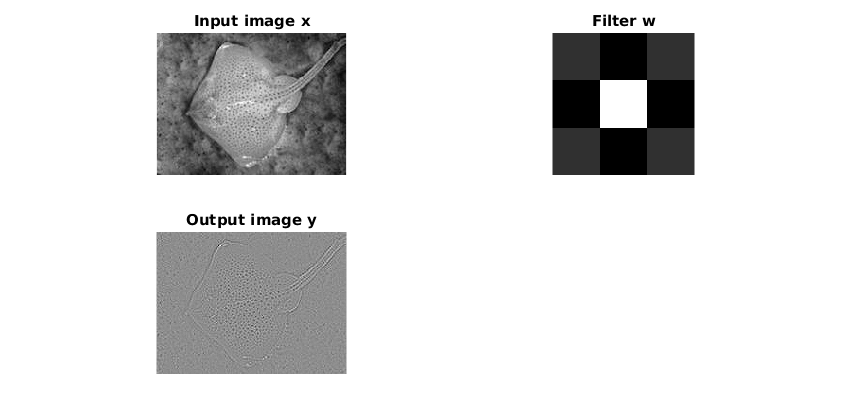
\includegraphics[width=0.8\textwidth]{conv}
 \caption{Gradient magnitude for different methods}
 \label{fig:q1}
\end{figure}

\paragraph{Question 1: If H x W is the size of the input image, H' x W' the size of the filter, what is the size H'' x W'' of the output image? Why?}
Different strategies apply giving different results. If only using the valid part of the image, no zero-padding, the resulting size is H''=H-(H'-1) x W''=W-(W'-1) because the value cannot be computed in the edges as there is no value to use when applying the kernel.
\paragraph{Question 2: The filter w given above is a discretized Laplacian operator. Which type of visual structures (corners, bars, ...) do you think may excite this filter the most?}
It will excite the most the edges, colour level discontinuities in the image.
\paragraph{Task 1: Suggest a way that you can make the output size be same as the input image size? Apply your suggestion using vl\_nnconv.}
Using zero padding around the image so the image edges have values around it that allow to compute the operation. y = vl\_nnconv(x, w, [],'Pad',1) ; Adds padding around the pixels of the input image before operating.

\subsection{Convolution by a filter bank}
\paragraph{Question 3: What is the number of feature channels K in this example? Why?} The number of feature channels is 3, one for each of the filters in the filter bank.
\paragraph{Task 2: Run the code above and visualize the individual feature channels in the tensor y by using the provided function showFeatureChannels(). Do the channel responses make sense given the
filter used to generate them?} Feature channel 1 shows the same result as in previous section. Feature channel 2 enhances more the vertical edges while feature channel 3 the horizontal.
\paragraph{Task 3: Implement the Sobel kernel as another channel and compare the results. Do you see any difference? Explain.} The difference is difficult to see but computing it and showing the result shows that there is a difference, mainly in the center of the edges which seem to be more 
\end{document}

